
%(BEGIN_QUESTION)
% Copyright 2006, Tony R. Kuphaldt, released under the Creative Commons Attribution License (v 1.0)
% This means you may do almost anything with this work of mine, so long as you give me proper credit

Elektriske motorer roterer vanligvis med for høy hastighet til å brukes direkte som ventilaktuatorer. Nesten alle elektriske ventilaktuatorer bruker girmekanismer for å redusere hastigheten på den elektriske motoren (og multiplisere dreiemomentet). En av de mest populære girmekanismene for å oppnå stor hastighetsreduksjon (og momentmultiplikasjon) kalles et {\it snekkegear}:

$$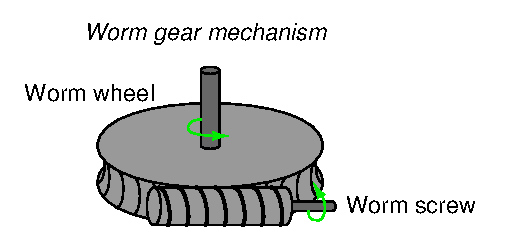
\includegraphics[width=8cm]{i01390x01.eps}$$

Tennene i snekkehjulet følger stigningen på gjengene i snekkeskruen, slik at de to delene griper inn i hverandre som tannhjul. Det bør være tydelig ved inspeksjon at det kreves svært mange omdreininger av snekkeskruen for å få én omdreining av snekkehjulet. I elektriske ventilaktuatorer er motoren koblet til snekkeskruen, og hjulet driver ventilmekanismen.

Det som kanskje ikke er like tydelig, er hvordan dreiemoment på snekkehjulet direkte omsettes til lineær skyvekraft i snekkeskruen. Med andre ord: Jo større vridende kraft som leveres av snekkehjulet, desto større rettlinjet kraft opplever skruen:

$$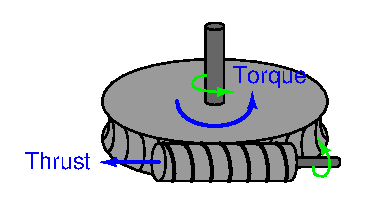
\includegraphics[width=8cm]{i01390x02.eps}$$

Hvis vi finner en måte å måle denne lineære skyvekraften i snekkeskruen på, kan vi utlede dreiemomentet fra hjulet. Forklar hvordan dette kan gjøres i en elektrisk ventilaktuator-mekanisme.

\underbar{file i01390}
%(END_QUESTION)





%(BEGIN_ANSWER)

En måte å måle aksialkraften i snekkeskruen på er med en {\it lastcelle}. En annen måte er å fjærbelaste skrueakselen og bruke en LVDT eller annen bevegelsessensor for å måle forskyvning.
 
%(END_ANSWER)





%(BEGIN_NOTES)

Dette er en vanlig måte å måle dreiemoment i mekanismer for elektriske ventilaktuatorer.

%INDEX% Final Control Elements, valve: electric actuator
%INDEX% Machine, gear (worm)

%(END_NOTES)

